\documentclass[12pt]{article}
\usepackage[utf8]{inputenc}
\usepackage[utf8]{inputenc}
\usepackage{amsmath}
\usepackage{amsthm}
\usepackage{geometry}
\usepackage{amsfonts}
\usepackage{mathrsfs}
\usepackage{bm}
\usepackage{hyperref}
\usepackage[dvipsnames]{xcolor}
\usepackage[inline]{enumitem}
\usepackage{mathtools}
\usepackage{changepage}
\usepackage{lipsum}
\usepackage{tikz}
\usetikzlibrary{matrix, patterns, decorations.pathreplacing, calligraphy}
\usepackage{tikz-cd}
\usepackage[nameinlink]{cleveref}
\geometry{
headheight=15pt,
left=60pt,
right=60pt
}
\setlength{\emergencystretch}{20pt}
\usepackage{fancyhdr}
\pagestyle{fancy}
\fancyhf{}
\lhead{}
\chead{Section 3.4 Exercises}
\rhead{\thepage}
\hypersetup{
    colorlinks=true,
    linkcolor=blue,
    urlcolor=blue
}

\theoremstyle{definition}
\newtheorem*{remark}{Remark}

\newtheoremstyle{exercise}
    {}
    {}
    {}
    {}
    {\bfseries}
    {.}
    { }
    {\thmname{#1}\thmnumber{#2}\thmnote{ (#3)}}
\theoremstyle{exercise}
\newtheorem{exercise}{Exercise 3.4.}

\newtheoremstyle{solution}
    {}
    {}
    {}
    {}
    {\itshape\color{magenta}}
    {.}
    { }
    {\thmname{#1}\thmnote{ #3}}
\theoremstyle{solution}
\newtheorem*{solution}{Solution}

\Crefformat{exercise}{#2Exercise 3.4.#1#3}

\newcommand{\interior}[1]{%
  {\kern0pt#1}^{\mathrm{o}}%
}
\newcommand{\ts}{\textsuperscript}
\newcommand{\setcomp}[1]{#1^{\mathsf{c}}}
\newcommand{\quand}{\quad \text{and} \quad}
\newcommand{\N}{\mathbf{N}}
\newcommand{\Z}{\mathbf{Z}}
\newcommand{\Q}{\mathbf{Q}}
\newcommand{\I}{\mathbf{I}}
\newcommand{\R}{\mathbf{R}}
\newcommand{\C}{\mathbf{C}}

\DeclarePairedDelimiter\abs{\lvert}{\rvert}
% Swap the definition of \abs* and \norm*, so that \abs
% and \norm resizes the size of the brackets, and the 
% starred version does not.
\makeatletter
\let\oldabs\abs
\def\abs{\@ifstar{\oldabs}{\oldabs*}}
%
\let\oldnorm\norm
\def\norm{\@ifstar{\oldnorm}{\oldnorm*}}
\makeatother

\setlist[enumerate,1]{label={(\alph*)}}

\begin{document}

\section{Section 3.4 Exercises}

Exercises with solutions from Section 3.4 of \hyperlink{ua}{[UA]}.

\begin{exercise}
\label{ex:1}
    If \( P \) is a perfect set and \( K \) is compact, is the intersection \( P \cap K \) always compact? Always perfect?
\end{exercise}

\begin{solution}
    \( P \) is closed, so \( P \cap K \) must be compact (\href{https://lew98.github.io/Mathematics/UA_Section_3_3_Exercises.pdf}{Exercise 3.3.4 (a)}). However, \( P \cap K \) need not be perfect. For a counterexample, consider \( P = [0, 1] \) and \( K = \{ 0 \} \).
\end{solution}

\begin{exercise}
\label{ex:2}
    Does there exist a perfect set consisting of only rational numbers?
\end{exercise}

\begin{solution}
    No. By Theorem 3.4.3, a non-empty perfect set must be uncountable, but any subset of \( \Q \) is either finite or countably infinite.
\end{solution}

\begin{exercise}
\label{ex:3}
    Review the portion of the proof given in Example 3.4.2 and follow these steps to complete the argument.
    \begin{enumerate}
        \item Because \( x \in C_1 \), argue that there exists an \( x_1 \in C \cap C_1 \) with \( x_1 \neq x \) satisfying \( \abs{x - x_1} \leq 1/3 \).

        \item Finish the proof by showing that for each \( n \in \N \), there exists \( x_n \in C \cap C_n \), different from \( x \) satisfying \( \abs{x - x_n} \leq 1/3^n \).
    \end{enumerate}
\end{exercise}

\begin{solution}
    \begin{enumerate}
        \item We have \( C_1 = [0, 1/3] \cup [2/3, 1] \). The endpoints of these intervals are never removed at any subsequent stage of the construction of the Cantor set, so they belong to \( C \). Since \( x \in C_1 \), it must belong to one of these intervals, say the interval \( [0, 1/3] \). If \( 0 \leq x < 1/3 \), then take \( x_1 = 1/3 \), and if \( x = 1/3 \), then take \( x_1 = 0 \). We can make similar choices if \( x \in [2/3, 1] \). In any case, we have chosen an \( x_1 \in C \cap C_1 \) with \( x_1 \neq x \) satisfying \( \abs{x - x_1} \leq 1/3 \).

        \item Let \( n \in \N \) be given. The set \( C_n \) consists of \( 2^n \) disjoint closed intervals each of length \( 1/3^n \). The endpoints of these intervals are never removed at any subsequent stage of the construction of the Cantor set, so they belong to \( C \). Since \( x \in C \), we have \( x \in C_n \) and hence \( x \) must belong to one of the disjoint closed intervals, say \( I = [a, b] \) where \( b - a = 1/3^n \). If \( a \leq x < b \), then let \( x_n = b \), and if \( x = b \) then let \( x_n = a \). In either case, we have chosen an \( x_n \in C \cap C_n \) such that \( x \neq x_n \) and \( \abs{x - x_n} \leq b - a = 1/3^n \).

        Thus \( x \) is the limit of a sequence \( (x_n) \) contained in \( C \) such that \( x_n \neq x \) for all \( n \in \N \). It follows that \( x \) is a limit point of \( C \) and hence that \( C \) contains no isolated points.
    \end{enumerate}
\end{solution}

\begin{exercise}
\label{ex:4}
    Repeat the Cantor construction from Section 3.1 starting with the interval \( [0, 1] \). This time, however, remove the open middle \textit{fourth} from each component.
    \begin{enumerate}
        \item Is the resulting set compact? Perfect?

        \item Using the algorithms from Section 3.1, compute the length and dimension of this Cantor-like set.
    \end{enumerate}
\end{exercise}

\begin{solution}
    We begin with \( B_0 := [0, 1] \) and remove the open middle fourth to obtain \( B_1 = \left[ 0, \tfrac{3}{8} \right] \cup \left[ \tfrac{5}{8}, 1 \right] \). Notice that each interval has length \( \tfrac{3}{8} \). Next we remove the open middle fourth from each of the two intervals of \( B_1 \) to obtain
    \[
        B_2 = \left( \left[ 0, \tfrac{9}{64} \right] \cup \left[ \tfrac{15}{64}, \tfrac{24}{64} \right] \right) \cup \left( \left[ \tfrac{40}{64}, \tfrac{49}{64} \right] \cup \left[ \tfrac{55}{64}, 1 \right] \right).
    \]
    Notice that each interval has length \( \left( \tfrac{3}{8} \right)^2 \). We continue in this fashion, obtaining sets \( B_n \) consisting of \( 2^n \) disjoint closed intervals each of length \( \left( \tfrac{3}{8} \right)^n \), and define our Cantor-like set \( B := \bigcap_{n=0}^{\infty} B_n \).
    \begin{enumerate}
        \item The set \( B \) is compact and perfect; the arguments used for the Cantor set work equally well for \( B \). Since each \( B_n \) is the finite union of closed sets, \( B_n \) is closed, and then since \( B \) is the intersection of closed sets, \( B \) is also closed. Clearly \( B \) is also bounded and hence \( B \) is compact. As in \Cref{ex:3}, given any \( x \in B \), we can find a sequence of endpoints \( (x_n) \) such that \( x_n \in B \cap B_n, x_n \neq x, \) and \( \abs{x - x_n} \leq \left( \tfrac{3}{8} \right)^n \) for each \( n \in \N \). It follows that \( x \) is a limit point of \( B \) and hence that \( B \) has no isolated points. Since \( B \) is also closed, we see that \( B \) is a perfect set.

        \item At the first stage, we remove an interval of length \( \tfrac{1}{4} \). At the \( n \)\ts{th} stage (\( n = 2, 3, 4 \ldots \)), we remove \( 2^{n-1} \) intervals each of length \( \tfrac{1}{4} \left( \tfrac{3}{8} \right)^{n-1} \). Thus the length of \( B \) is
        \[
            1 - \left( \tfrac{1}{4} + 2 \cdot \tfrac{1}{4} \cdot \tfrac{3}{8} + 2^2 \cdot \tfrac{1}{4} \cdot \left( \tfrac{3}{8} \right)^2 + \cdots \right) = 1 - \tfrac{1}{4} \left( 1 + \tfrac{3}{4} + \left( \tfrac{3}{4} \right)^2 + \cdots \right) = 1 - \frac{\tfrac{1}{4}}{1 - \tfrac{3}{4}} = 0.
        \]
        To calculate the dimension of \( B \), we magnify the set by a factor of \( \tfrac{8}{3} \), so that \( B_0 \) becomes the closed interval \( \left[ 0, \tfrac{8}{3} \right] \). Then when we remove the open middle fourth of this interval, we are left with two intervals of length 1:
        \[
            B_1 = [0, 1] \cup \left[ \tfrac{5}{3}, \tfrac{8}{3} \right].
        \]
        Thus we will obtain two copies of \( B \). Then the dimension \( x \) of \( B \) is given by solving \( 2 = \left( \tfrac{8}{3} \right)^x \), which gives
        \[
            x = \frac{\log(2)}{\log\left( \tfrac{8}{3} \right)} \approx 0.7067.
        \]
    \end{enumerate}
\end{solution}

\begin{exercise}
\label{ex:5}
    Let \( A \) and \( B \) be nonempty subsets of \( \R \). Show that if there exist disjoint open sets \( U \) and \( V \) with \( A \subseteq U \) and \( B \subseteq V \), then \( A \) and \( B \) are separated.
\end{exercise}

\begin{solution}
    Observe that \( \setcomp{V} \) is a closed set which contains \( A \) (since \( U \cap V = \emptyset \implies A \cap V = \emptyset \)). Since \( \overline{A} \) is the smallest closed set containing \( A \) (Theorem 3.2.12), we must have \( \overline{A} \subseteq \setcomp{V} \), which gives
    \[
        \overline{A} \subseteq \setcomp{V} \implies \overline{A} \cap V = \emptyset \implies \overline{A} \cap B = \emptyset.
    \]
    Similarly, \( A \cap \overline{B} = \emptyset \). Thus \( A \) and \( B \) are separated.
\end{solution}

\begin{exercise}
\label{ex:6}
    Prove Theorem 3.4.6.
\end{exercise}

\begin{solution}
    Suppose we have non-empty subsets \( A, B \subseteq \R \) such that every convergent sequence contained in one of the subsets has a limit which does not belong to the other subset. Since a limit point of \( A \) is the limit of a sequence contained in \( A \) and an element of \( A \) is the limit of a constant sequence contained in \( A \), and by assumption these limits do not belong to \( B \), we see that \( \overline{A} \cap B = \emptyset \). Similarly, \( A \cap \overline{B} = \emptyset \). Thus \( A \) and \( B \) are separated.

    Conversely, suppose that \( A \) and \( B \) are separated. If \( (x_n) \to x \) is a convergent sequence contained in \( A \), then \( x \in \overline{A} \). It follows that \( x \not\in B \) since \( \overline{A} \cap B = \emptyset \). Similarly, the limit of any convergent sequence contained in \( B \) must not belong to \( A \).

    We have now shown that for non-empty subsets \( A, B \subseteq \R \), \( A \) and \( B \) being separated is equivalent to the condition that every convergent sequence contained in one of the subsets has a limit which does not belong to the other subset.

    Proving Theorem 3.4.6 is equivalent to showing that a subset \( E \subseteq \R \) is disconnected if and only if there exist non-empty subsets \( A, B \subseteq E \) such that \( E = A \cup B \) and every convergent sequence contained in one of the subsets has a limit which does not belong to the other subset. By the previous discussion, such subsets are separated. So the theorem follows by the definition of disconnectedness.
\end{solution}

\begin{exercise}
\label{ex:7}
    A set \( E \) is \textit{totally disconnected} if, given any two distinct points \( x, y \in E \), there exist separated sets \( A \) and \( B \) with \( x \in A, y \in B \), and \( E = A \cup B \).
    \begin{enumerate}
        \item Show that \( \Q \) is totally disconnected.
        
        \item Is the set of irrational numbers totally disconnected?
    \end{enumerate}
\end{exercise}

\begin{solution}
    \begin{enumerate}
        \item Suppose that \( p < q \) are rational numbers. By the density of \( \I \) in \( \R \), there exists an irrational number \( y \) such that \( p < y < q \). Define the sets
        \[
            A = (-\infty, y) \cap \Q \quand B = (y, \infty) \cap \Q.
        \]
        Then \( p \in A, q \in B \), and since \( y \not\in \Q \), we have \( A \cup B = \Q \). By the density of \( \Q \) in \( \R \), we have \( \overline{A} = (-\infty, y] \) and \( \overline{B} = [y, \infty) \). It follows that \( \overline{A} \cap B = A \cap \overline{B} = \emptyset \) and hence that \( A \) and \( B \) are separated. Thus \( \Q \) is totally disconnected.

        \item \( \I \) is also totally disconnected. To see this, reverse the roles of \( \Q \) and \( \I \) in the solution to part (a).
    \end{enumerate}
\end{solution}

\begin{exercise}
\label{ex:8}
    Follow these steps to show that the Cantor set is totally disconnected in the sense described in \Cref{ex:7}.

    Let \( C = \bigcap_{n=0}^{\infty} C_n \), as defined in Section 3.1.
    \begin{enumerate}
        \item Given \( x, y \in C \), with \( x < y \), set \( \epsilon = y - x \). For each \( n = 0, 1, 2, \ldots, \) the set \( C_n \) consists of a finite number of closed intervals. Explain why there must exist an \( N \) large enough so that it is impossible for \( x \) and \( y \) both to belong to the same closed interval of \( C_N \).

        \item Show that \( C \) is totally disconnected.
    \end{enumerate}
\end{exercise}

\begin{solution}
    \begin{enumerate}
        \item If \( I \) is an interval of length \( \delta \), then any \( a, b \in I \) must satisfy \( \abs{a - b} \leq \delta \). In the construction of \( C \), each \( C_n \) consists of \( 2^n \) disjoint closed intervals each of length \( 3^{-n} \). Thus we can find an \( N \) large enough so that \( C_N \) consists of closed intervals each of length \( 3^{-N} < \epsilon = y - x \), i.e.\ whose length is smaller than the distance between \( x \) and \( y \). Then \( x \) and \( y \) cannot possibly belong to the same interval of \( C_N \).

        \item Let \( [a, b] \) be the closed interval of \( C_N \) which contains \( x \) and note that the open interval \( \left( b, b + \tfrac{1}{3^N} \right) \) was either removed at the \( N \)\ts{th} stage of construction or is a subset of an open interval which was removed at a previous stage of construction. So if we set \( t := b + \tfrac{1}{2 \cdot 3^N} \), then \( t \not\in C \). Since \( y \not\in [a, b] \) and \( y > x \), we must have \( y > t \). Define
        \[
            A = (-\infty, t) \cap C \quand B = (t, \infty) \cap C.  
        \]
        Then \( x \in A, y \in B \), and since \( t \not\in C \), we have \( A \cup B = C \). If \( (z_n) \to z \) is a convergent sequence contained in \( A \), then the Order Limit Theorem implies that \( z \leq t \) and hence that \( z \not\in B \). Similarly, the limit of any convergent sequence contained in \( B \) cannot belong to \( A \). Thus \( A \) and \( B \) are separated by Theorem 3.4.6 (see \Cref{ex:6}). It follows that \( C \) is totally disconnected.
    \end{enumerate}
\end{solution}

\begin{exercise}
\label{ex:9}
    Let \( \{ r_1, r_2, r_3, \ldots \} \) be an enumeration of the rational numbers, and for each \( n \in \N \) set \( \epsilon_n = 1/2^n \). Define \( O = \bigcup_{n=1}^{\infty} V_{\epsilon_n}(r_n) \) and let \( F = \setcomp{O} \).
    \begin{enumerate}
        \item Argue that \( F \) is a closed, nonempty set consisting only of irrational numbers.

        \item Does \( F \) contain any nonempty open intervals? Is \( F \) totally disconnected? (See \Cref{ex:7} for the definition.)

        \item Is it possible to know whether \( F \) is perfect? If not, can we modify this construction to produce a nonempty perfect set of irrational numbers?
    \end{enumerate}
\end{exercise}

\begin{solution}
    \begin{enumerate}
        \item \( O \) is an open set since it is a union of open intervals, so \( F = \setcomp{O} \) must be closed. To see that \( F \) is non-empty, suppose otherwise. Then \( O = \R \), so the collection \( \{ V_{\epsilon_n}(r_n) : n \in \N \} \) is an open cover of the compact set \( [0, 10] \). Thus there exist finitely many indices \( n_1 < \cdots < n_K \) such that
        \[
            [0, 10] \subseteq V_{\epsilon_{n_1}}(r_{n_1}) \cup \cdots \cup V_{\epsilon_{n_K}}(r_{n_K}).
        \]
        However, the interval \( [0, 10] \) has length 10, whereas the set \( V_{\epsilon_{n_1}}(r_{n_1}) \cup \cdots \cup V_{\epsilon_{n_K}}(r_{n_K}) \) has total length at most
        \[
            \sum_{k=1}^K \frac{1}{2^{n_k - 1}} \leq \sum_{k=0}^{\infty} \frac{1}{2^k} = 2,
        \]
        since \( \abs{V_{\epsilon_{n_k}}(r_{n_k})} = 2 \epsilon_{n_k} = 1/2^{n_k - 1} \). So we have a set of length 10 contained inside a set of length 2, which is a contradiction. Thus \( F \) is non-empty. Clearly, \( \Q \subseteq O \), so \( F = \setcomp{O} \) can contain only irrational numbers.

        \item \( F \) cannot contain any non-empty open intervals, since this would imply that \( F \) contains a rational number (indeed, infinitely many rational numbers), but by part (a) \( F \) contains only irrational numbers.

        To see that \( F \) is totally disconnected, let us show that any subset of a totally disconnected set is also totally disconnected. Suppose we have sets \( E \subseteq G \subseteq \R \) such that \( G \) is totally disconnected. Let \( x, y \in E \) be given. Then since \( x \) and \( y \) belong to the totally disconnected set \( G \), there exist separated sets \( A \) and \( B \) such that \( x \in A, y \in B, \) and \( G = A \cup B \). Set \( A' = A \cap E \) and \( B' = B \cap E \) and note that \( x \in A' \) and \( y \in B' \). Furthermore, \( A' \subseteq A \) and \( B' \subseteq B \), so
        \[
            \overline{A'} \subseteq \overline{A} \implies \overline{A'} \cap B' \subseteq \overline{A} \cap B' \subseteq \overline{A} \cap B = \emptyset.
        \]
        Thus \( \overline{A'} \cap B' = \emptyset \), and similarly \( A' \cap \overline{B'} = \emptyset \), so that \( A' \) and \( B' \) are separated. Finally,
        \[
            E = E \cap G = E \cap (A \cup B) = (A \cap E) \cup (B \cap E) = A' \cup B'.
        \]
        It follows that \( E \) is totally disconnected.
        
        Since \( F \) is a subset of \( \I \), which we showed was totally disconnected in \Cref{ex:7}, by the previous paragraph we have that \( F \) is totally disconnected.

        \item There are enumerations of \( \Q \) which, when used in this construction, will result in an \( F \) which is not perfect, i.e.\ an \( F \) with at least one isolated point. We will construct such an enumeration \( (r_n) \), which gives an \( F \) with \( \sqrt{2} \) as an isolated point, via the following four step process. (Any irrational number would also work in place of \( \sqrt{2} \).)
        \begin{description}
            \item[Step 1.] We will first construct a strictly increasing sequence \( (p_n) \) of distinct rational numbers such that:
            \begin{enumerate}[itemsep=8pt, leftmargin=44pt, label=(1.\arabic*)]
                \item \( p_1 < p_2 < p_3 < \cdots < \sqrt{2} \);

                \item \( \left( \sqrt{2} - \tfrac{1}{16}, \sqrt{2} \right) \subseteq \bigcup_{n=1}^{\infty} V_{\epsilon_{4n}}(p_n) \);

                \item \( \sqrt{2} \not\in \bigcup_{n=1}^{\infty} V_{\epsilon_{4n}}(p_n) \).
            \end{enumerate}
            This sequence will be placed in the final enumeration \( (r_n) \) as \( r_{4n} = p_n \), so that
            \[
                r_4 = p_1, r_8 = p_2, r_{12} = p_3, \ldots
            \]

            \item[Step 2.] Mirroring Step 1, we will construct a strictly decreasing sequence \( (q_n) \) of distinct rational numbers such that:
            \begin{enumerate}[itemsep=8pt, leftmargin=44pt, label=(2.\arabic*)]
                \item \( \sqrt{2} < \cdots < q_3 < q_2 < q_1 \);

                \item \( \left( \sqrt{2}, \sqrt{2} + \tfrac{1}{16} \right) \subseteq \bigcup_{n=1}^{\infty} V_{\epsilon_{4n-2}}(q_n) \);

                \item \( \sqrt{2} \not\in \bigcup_{n=1}^{\infty} V_{\epsilon_{4n-2}}(q_n) \).
            \end{enumerate}
            This sequence will be placed in the final enumeration \( (r_n) \) as \( r_{4n-2} = q_n \), so that
            \[
                r_2 = q_1, r_6 = q_2, r_{10} = q_3, \ldots
            \]

            \item[Step 3.] There are infinitely many rational numbers which belong to neither of the sequences \( (p_n) \) nor \( (q_n) \) from Steps 1 and 2. We will construct a sequence \( (a_n) \) which enumerates these remaining rational numbers in such a way that \( \sqrt{2} \) will not be excluded from \( F \) in the final construction, i.e.\ a sequence \( (a_n) \) such that:
            \begin{enumerate}[itemsep=8pt, leftmargin=44pt, label=(3.\arabic*)]
                \item \( a_m \neq a_n \) for \( m \neq n \);

                \item for each rational \( r \in \setcomp{(\{ p_1, p_2, \ldots \} \cup \{ q_1, q_2, \ldots \})}, \) there exists an \( n \in \N \) such that \( a_n = r \).

                \item \( \sqrt{2} \not\in \bigcup_{n=1}^{\infty} V_{\epsilon_{2n-1}}(a_n) \).
            \end{enumerate}
            This sequence will be placed in the final enumeration \( (r_n) \) as \( r_{2n-1} = a_n \), so that
            \[
                r_1 = a_1, r_3 = a_2, r_5 = a_3, \ldots
            \]

            \item[Step 4.] We will combine the sequences \( (p_n), (q_n), \) and \( (a_n) \) to obtain an enumeration \( (r_n) \) of \( \Q \) given by
            \[
                a_1, q_1, a_2, p_1, a_3, q_2, a_4, p_2, \ldots
            \]
            Letting \( O = \bigcup_{n=1}^{\infty} V_{\epsilon_n}(r_n) \) and \( F = \setcomp{O} \), we will have
            \[
                \left( \sqrt{2} - \tfrac{1}{16}, \sqrt{2} \right) \cup \left( \sqrt{2}, \sqrt{2} + \tfrac{1}{16} \right) \subseteq O \quand \sqrt{2} \not\in O,
            \]
            so that \( \left( \sqrt{2} - \tfrac{1}{16}, \sqrt{2} + \tfrac{1}{16} \right) \cap F = \left\{ \sqrt{2} \right\} \). Thus \( \sqrt{2} \) will be an isolated point of \( F \).
        \end{description}

        \noindent \hrulefill

        {\Large \textbf{Step 1.}}

        For each \( n \in \N \), let \( p_n \) be a rational number satisfying
        \[
            \sqrt{2} - \frac{1}{2^{4n}} - \frac{1}{2^{4n + 4}} < p_n < \sqrt{2} - \frac{1}{2^{4n}};
        \]
        the existence of such a rational number is guaranteed by the density of \( \Q \) in \( \R \). Observe that for each \( n \in \N \) we have
        \[
            p_n < \sqrt{2} - \frac{1}{2^{4n}} < \sqrt{2} - \frac{1}{2^{4n+4}} - \frac{1}{2^{4n + 8}} < p_{n+1} \quand p_n < \sqrt{2}.
        \]
        Thus the sequence \( (p_n) \) satisfies condition (1.1).
        
        For any \( n \in \N \) we have
        \[
            p_n < p_{n+1} < \sqrt{2} - \frac{1}{2^{4n + 4}} < p_n + \frac{1}{2^{4n}} < \sqrt{2},
        \]
        so that \( p_{n+1} \in (p_n, p_n + 2^{-4n}) \subseteq V_{\epsilon_{4n}}(p_n) \), i.e.\ the centre of \( V_{\epsilon_{4n+4}}(p_{n+1}) \) is contained in \( V_{\epsilon_{4n}}(p_n) \). Thus, for any \( N \in \N \), the union \( \bigcup_{n=1}^N V_{\epsilon_{4n}}(p_n) \) must be an open interval:
        \[
            \bigcup_{n=1}^N V_{\epsilon_{4n}}(p_n) = \left( p_1 - \tfrac{1}{16}, B \right),
        \]
        where \( B = \max \{ p_n + \tfrac{1}{2^{4n}} : 1 \leq n \leq N \} \) (the exact value of \( B \) is not particularly important, but note that it must be strictly less than \( \sqrt{2} \)). Since
        \[
            p_1 < \sqrt{2} - \frac{1}{16} < p_1 + \frac{1}{16},
        \]
        we have \( \sqrt{2} - \tfrac{1}{16} \in \bigcup_{n=1}^N V_{\epsilon_{4n}}(p_n) \) for any \( N \in \N \). Let \( y \in \R \) be such that \( \sqrt{2} - \tfrac{1}{16} < y < \sqrt{2} \). Since \( (p_n) \) is increasing and converges to \( \sqrt{2} \), we can find an \( N \in \N \) such that \( y < p_N < \sqrt{2} \). Then since \( \sqrt{2} - \tfrac{1}{16} \) and \( p_N \) both belong to the open interval \( \bigcup_{n=1}^N V_{\epsilon_{4n}}(p_n) \) and \( y \) lies between these two values, we must have \( y \in \bigcup_{n=1}^N V_{\epsilon_{4n}}(p_n) \) and thus \( y \in \bigcup_{n=1}^{\infty} V_{\epsilon_{4n}}(p_n) \). Hence the sequence \( (p_n) \) satisfies condition (1.2).

        Finally, as noted above we have \( p_n + 2^{-4n} < \sqrt{2} \) for all \( n \in \N \), so the sequence \( (p_n) \) also satisfies condition (1.3).

        \noindent \hrulefill

        {\Large \textbf{Step 2.}}

        The construction of the sequence \( (q_n) \) is analogous to the construction given in Step 1; for each \( n \in \N \), let \( q_n \) be a rational number satisfying
        \[
            \sqrt{2} + \frac{1}{2^{4n - 2}} < q_n <  \sqrt{2} + \frac{1}{2^{4n - 2}} + \frac{1}{2^{4n + 2}};
        \]
        the existence of such a rational number is guaranteed by the density of \( \Q \) in \( \R \). Similar logic to that given in Step 1 shows that the sequence \( (q_n) \) satisfies condition (2.1), and furthermore that \( \left( \sqrt{2}, \sqrt{2} + \tfrac{1}{4} \right) \subseteq \bigcup_{n=1}^{\infty} V_{\epsilon_{4n-2}}(q_n) \), which gives us condition (2.2). Condition (2.3) follows since \( \sqrt{2} < q_n - \tfrac{1}{2^{4n - 2}} \) for all \( n \in \N \).

        \noindent \hrulefill

        {\Large \textbf{Step 3.}}

        Since the sequences \( (p_n) \) and \( (q_n) \) constructed in Steps 1 and 2 are entirely contained inside the interval \( [p_1, q_1] \), it is clear that there are infinitely many rational numbers left to enumerate. That is, letting
        \[
            E = \Q \cap \setcomp{(\{ p_1, p_2, \ldots \} \cup \{ q_1, q_2, \ldots \})},
        \]
        we have that \( E \) is countably infinite. However, enumerating \( E \) carelessly might exclude \( \sqrt{2}\) from \( F \) in Step 4, since there are rational numbers in \( E \) arbitrarily close to \( \sqrt{2} \); placing one of these rational numbers ``too early'' in the sequence \( (r_n) \) will include \( \sqrt{2} \) in some \( V_{\epsilon_n}(r_n) \). To surmount this problem, we will first partition \( E \) as follows. Let
        \[
            A_n = \begin{cases}
                \left\{ x \in \R : \epsilon_1 < \abs{x - \sqrt{2}} \right\} & \text{if } n = 1, \\
                \left\{ x \in \R : \epsilon_{2n - 1} < \abs{x - \sqrt{2}} < \epsilon_{2n - 3} \right\} & \text{if } n \geq 2.
            \end{cases}
        \]
        Equivalently,
        \[
            A_n = \begin{cases}
                \left( -\infty, \sqrt{2} - \epsilon_1 \right) \cup \left( \sqrt{2} + \epsilon_1, \infty \right) & \text{if } n = 1, \\
                \left( \sqrt{2} - \epsilon_{2n - 3}, \sqrt{2} - \epsilon_{2n - 1} \right) \cup \left( \sqrt{2} + \epsilon_{2n - 1}, \sqrt{2} + \epsilon_{2n - 3} \right) & \text{if } n \geq 2.
            \end{cases}
        \]
        Now set \( E_n = E \cap A_n \) for each \( n \in \N \).
        \begin{figure}[h]
            \centering
            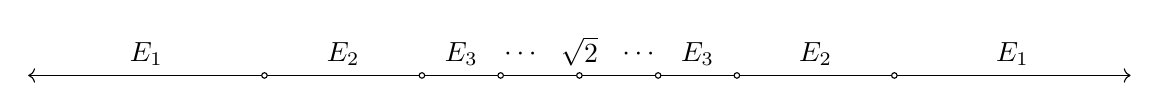
\begin{tikzpicture}
                \draw[<->] (-7, 0) -- (7, 0);
                \filldraw[draw=black, fill=white]
                    (0, 0) circle (1pt) node [anchor=south] {\( \sqrt{2} \)}
                    (-1, 0) circle (1pt)
                    (-2, 0) circle (1pt)
                    (-4, 0) circle (1pt)
                    (1, 0) circle (1pt)
                    (2, 0) circle (1pt)
                    (4, 0) circle (1pt);
                \path
                    (-5.5, 0) node [anchor=south] {\( E_1 \)}
                    (5.5, 0) node [anchor=south] {\( E_1 \)}
                    (-3, 0) node [anchor=south] {\( E_2 \)}
                    (3, 0) node [anchor=south] {\( E_2 \)}
                    (-1.5, 0) node [anchor=south] {\( E_3 \)}
                    (1.5, 0) node [anchor=south] {\( E_3 \)}
                    (-0.75, 0) node [anchor=south, yshift=2pt] {\( \cdots \)}
                    (0.75, 0) node [anchor=south, yshift=2pt] {\( \cdots \)};
            \end{tikzpicture}
            \caption{Partition of \( E \)} \label{fig:1}
        \end{figure}
        
        We have \( \bigcup_{n=1}^{\infty} E_n = E \) since the only real numbers not contained in \( \bigcup_{n=1}^{\infty} A_n \) are \( \sqrt{2} \) and those of the form \( \sqrt{2} \pm \epsilon_{2n - 1} \) for some \( n \in \N \), none of which are rational. Then since the collection \( \{ E_n : n \in \N \} \) is evidently pairwise disjoint, we have a partition of \( E \).

        Since \( \lim_{n \to \infty} p_n = \lim_{n \to \infty} q_n = \sqrt{2} \) and \( \sqrt{2} \not\in \overline{A_n} \) for any \( n \in \N \), we see that there can be only finitely many terms of the sequences \( (p_n) \) and \( (q_n) \) contained in each \( A_n \); it follows that each \( E_n \) is countably infinite. We can then enumerate each \( E_n \):
        \[
            E_n = \{ e_{1,n}, e_{2,n}, e_{3,n}, \ldots \}.
        \]
        These enumerations can be combined to form an enumeration \( (a_n) \) of \( E \) using the same diagonal method as that used in the proof that a countable union of countable sets is itself countable (see, for example, \href{https://lew98.github.io/Mathematics/UA_Section_1_5_Exercises.pdf}{Exercise 1.5.3 (c)}). To be precise, consider the following ``infinite arrays''.
        \[
            \begin{matrix}
            e_{1,1} & e_{1,2} & e_{1,3} & e_{1,4} & e_{1,5} & \cdots \\
            e_{2,1} & e_{2,2} & e_{2,3} & e_{2,4} & \ddots &  \\
            e_{3,1} & e_{3,2} & e_{3,3} & \ddots &  &  \\
            e_{4,1} & e_{4,2} & \ddots &   &  &  \\
            e_{5,1} & \ddots &  &  &  &  \\
            \vdots &  &  &  &  & 
            \end{matrix}
            \qquad
            \begin{matrix}
            a_1 & a_3 & a_6 & a_{10} & a_{15} & \cdots \\
            a_2 & a_5 & a_9 & a_{14} & \ddots &  \\
            a_4 & a_8 & a_{13} & \ddots &  &  \\
            a_7 & a_{12} & \ddots &   &  &  \\
            a_{11} & \ddots &  &  &  &  \\
            \vdots &  &  &  &  & 
            \end{matrix}
        \]
        The enumeration of \( E_n \) is the \( n \)\ts{th} column of the left-hand array. The enumeration of \( E \) is obtained by letting \( a_N \) in the right-hand array be the element \( e_{m,n} \) in the corresponding position of the left-hand array, so that
        \[
            a_1 = e_{1,1}, a_2 = e_{2,1}, a_3 = e_{1,2}, a_4 = e_{3,1}, \ldots
        \]
        This mapping is bijective because the collection \( \{ E_n : n \in \N \} \) is a partition of \( E \). Thus the sequence \( (a_n) \) satisfies conditions (3.1) and (3.2).

        To show that the sequence \( (a_n) \) satisfies condition (3.3), we need to show that for all \( n \in \N, \sqrt{2} \not\in V_{\epsilon_{2n - 1}}(a_n) \). Let \( n \in \N \) be given. Then \( a_n \) belongs to some column of the right-hand array above, say the \( N \)\ts{th} column. From the definition of our enumeration \( (a_n) \), we have \( a_n = e_{m,N} \) for some \( m \in \N \). It follows that \( a_n \in E_N \) and hence that \( \abs{a_n - \sqrt{2}} > \epsilon_{2N - 1} \), which gives \( \sqrt{2} \not\in V_{\epsilon_{2N - 1}}(a_n) \).
        
        If we examine the right-hand array, we see that the element at the top of the \( N \)\ts{th} column is \( a_{N(N+1)/2} \) (the \( N \)\ts{th} triangular number), and furthermore that \( n \geq N(N+1)/2 \). Then
        \[
            2n - 1 \geq N(N+1) - 1 \geq 2N - 1 \implies \epsilon_{2n-1} \leq \epsilon_{2N-1} \implies V_{\epsilon_{2n - 1}}(a_n) \subseteq V_{\epsilon_{2N - 1}}(a_n).
        \]
        Combining this with \( \sqrt{2} \not\in V_{\epsilon_{2N - 1}}(a_n) \), we see that \( \sqrt{2} \not\in V_{\epsilon_{2n - 1}}(a_n) \). Thus the sequence \( (a_n) \) satisfies condition (3.3).

        \noindent \hrulefill

        {\Large \textbf{Step 4.}}

        We can now form our final enumeration \( (r_n) \), by setting
        \[
            r_{2n-1} = a_n, \quad r_{4n-2} = q_n, \quand r_{4n} = p_n,
        \]
        so that \( (r_n) \) is the sequence
        \[
                a_1, q_1, a_2, p_1, a_3, q_2, a_4, p_2, \ldots
        \]
        Let \( O = \bigcup_{n=1}^{\infty} V_{\epsilon_n}(r_n) \) and \( F = \setcomp{O} \). By condition (1.2), we have
        \[
            \left( \sqrt{2} - \tfrac{1}{16}, \sqrt{2} \right) \subseteq \bigcup_{n=1}^{\infty} V_{\epsilon_{4n}}(p_n) = \bigcup_{n=1}^{\infty} V_{\epsilon_{4n}}(r_{4n}) \subseteq \bigcup_{n=1}^{\infty} V_{\epsilon_n}(r_n) = O,
        \]
        and by condition (2.2), we have
        \[
            \left( \sqrt{2}, \sqrt{2} + \tfrac{1}{16} \right) \subseteq \bigcup_{n=1}^{\infty} V_{\epsilon_{4n-2}}(q_n) = \bigcup_{n=1}^{\infty} V_{\epsilon_{4n-2}}(r_{4n-2}) \subseteq \bigcup_{n=1}^{\infty} V_{\epsilon_n}(r_n) = O.
        \]
        Thus \( \left( \sqrt{2} - \tfrac{1}{16}, \sqrt{2} \right) \cup \left( \sqrt{2}, \sqrt{2} + \tfrac{1}{16} \right) \subseteq O \). Furthermore, since
        \begin{align*}
            O &= \bigcup_{n=1}^{\infty} V_{\epsilon_n}(r_n) \\
            &= \bigcup_{n=1}^{\infty} V_{\epsilon_{4n}}(r_{4n}) \cup \bigcup_{n=1}^{\infty} V_{\epsilon_{4n-2}}(r_{4n-2}) \cup \bigcup_{n=1}^{\infty} V_{\epsilon_{2n-1}}(r_{2n-1}) \\
            &= \bigcup_{n=1}^{\infty} V_{\epsilon_{4n}}(p_n) \cup \bigcup_{n=1}^{\infty} V_{\epsilon_{4n-2}}(q_n) \cup \bigcup_{n=1}^{\infty} V_{\epsilon_{2n-1}}(a_n),
        \end{align*}
        conditions (1.3), (2.3), and (3.3) imply that \( \sqrt{2} \not\in O \). It follows that
        \[
            \left( \sqrt{2} - \tfrac{1}{16}, \sqrt{2} + \tfrac{1}{16} \right) \cap F = \left\{ \sqrt{2} \right\}.
        \]
        Then \( \sqrt{2} \) is an isolated point of \( F \) and thus \( F \) is not a perfect set.

        \noindent \hrulefill

        Regarding the second half of the question, it is possible to modify the construction to produce a non-empty perfect set consisting of only irrational numbers. To do this, we start with any enumeration \( (r_n) \) of \( \Q \) and inductively define a sequence of non-negative real numbers \( (\epsilon_n) \) in such a way that if we set
        \[
            O = \bigcup_{n=1}^{\infty} V_{\epsilon_n}(r_n) \quand F = \setcomp{O},
        \]
        then \( F \) will be a non-empty perfect of irrational numbers. Intuitively, we will inductively construct \( O \) as a union of disjoint open intervals, with no pair of these intervals sharing an endpoint. (In what follows, we adopt the convention that \( V_{\epsilon}(x) = \emptyset \) if \( \epsilon = 0 \).)

        Suppose that after \( N \) steps we have chosen \( \epsilon_1, \ldots, \epsilon_N \) such that:
        \begin{enumerate}[leftmargin=40pt, label=(IH\arabic*)]
            \item \( \{ r_1, \ldots, r_N \} \subseteq \bigcup_{n=1}^{N} V_{\epsilon_n}(r_n) \);

            \item for all \( 1 \leq n \leq N \), either \( \epsilon_n = 0 \) or \( \epsilon_n \) is positive, irrational, and satisfies \( \epsilon_n \leq \tfrac{\sqrt{2}}{2^n} \);

            \item \( \overline{V_{\epsilon_m}(r_m)} \cap \overline{V_{\epsilon_n}(r_n)} = \emptyset \) for all \( m, n \in \N \) with \( 1 \leq m < n \leq N \).
        \end{enumerate}
        
        Let \( U = \bigcup_{n=1}^N V_{\epsilon_n}(r_n) \). There are two cases.
        \begin{description}
            \item[Case 1.] This is the easier case. If \( r_{N+1} \in U \), then set \( \epsilon_{N+1} = 0 \), so that \( V_{\epsilon_{N+1}}(r_{N+1}) = \emptyset \). (IH1) combined with \( r_{N+1} \in U \) gives us
            \[
                \{ r_1, \ldots, r_N, r_{N+1} \} \subseteq U = \bigcup_{n=1}^N V_{\epsilon_n}(r_n) = \bigcup_{n=1}^{N+1} V_{\epsilon_n}(r_n),
            \]
            where the last equality follows from \( V_{\epsilon_{N+1}}(r_{N+1}) = \emptyset \).
            
            Combining (IH2) with \( \epsilon_{N+1} = 0 \), we see that for all \( 1 \leq n \leq N + 1 \), either \( \epsilon_n = 0 \) or \( \epsilon_n \) is positive, irrational, and satisfies \( \epsilon_n \leq \tfrac{\sqrt{2}}{2^n} \).

            Similarly, combining (IH3) with \( V_{\epsilon_{N+1}}(r_{N+1}) = \emptyset \), we have \( \overline{V_{\epsilon_m}(r_m)} \cap \overline{V_{\epsilon_n}(r_n)} = \emptyset \) for all \( m, n \in \N \) with \( 1 \leq m < n \leq N + 1 \).

            \item[Case 2.] This is the harder case. If \( r_{N+1} \not\in U \) then let \( \epsilon_{n_1}, \ldots, \epsilon_{n_J} \) be those \( \epsilon \)'s from \( \epsilon_1, \ldots, \epsilon_N \) which are non-zero; there must be at least one such \( \epsilon_{n_j} \) by (IH1) and each \( \epsilon_{n_j} \) must be positive and irrational by (IH2). Observe that
            \[
                U = \bigcup_{n=1}^N V_{\epsilon_n}(r_n) = \bigcup_{j=1}^J V_{\epsilon_{n_j}}(r_{n_j}),
            \]
            where each \( V_{\epsilon_{n_j}}(r_{n_j}) \) is a proper open interval. For each \( 1 \leq j \leq J \), note that since \( r_{N+1} \not\in U \), we must have \( r_{N+1} \not\in V_{\epsilon_{n_j}}(r_{n_j}) \). Both of the endpoints of \( V_{\epsilon_{n_j}}(r_{n_j}) \) are the sum of a rational number and an irrational number and hence are irrational; since \( r_{N+1} \) is rational, we see that \( r_{N+1} \not\in [r_{n_j} - \epsilon_{n_j}, r_{n_j} + \epsilon_{n_j}] \). Given this, if we let \( d \) be the minimum of the distances from \( r_{N+1} \) to the endpoints of each \( V_{\epsilon_{n_j}} \), i.e.\
            \[
                d = \min \left\{ \abs{r_{n_j} - \epsilon_{n_j} - r_{N+1}}, \abs{r_{n_j} + \epsilon_{n_j} - r_{N+1}} : 1 \leq j \leq J \right\},
            \]
            then \( d \) must be positive. Furthermore, \( d \) must be irrational since it is the sum of a rational number and an irrational number, and for each \( 1 \leq j \leq J \), we have
            \begin{equation}
                \left[ r_{N+1} - \tfrac{d}{2}, r_{N+1} + \tfrac{d}{2} \right] \cap [r_{n_j} - \epsilon_{n_j}, r_{n_j} + \epsilon_{n_j}] = \emptyset.
            \end{equation}

            Set \( \epsilon_{N+1} = \min \left\{ \tfrac{\sqrt{2}}{2^{N+1}}, \tfrac{d}{2} \right\} \). Then \( \epsilon_{N+1} \) is positive, so \( r_{N+1} \in V_{\epsilon_{N+1}}(r_{N+1}) \). Combining this with (IH1) gives us
            \[
                \{ r_1, \ldots, r_N, r_{N+1} \} \subseteq \bigcup_{n=1}^{N+1} V_{\epsilon_n}(r_n).
            \]
            As noted before, \( d \) is positive and irrational, so \( \epsilon_{N+1} \) is positive, irrational, and satisfies \( \epsilon_{N+1} \leq \tfrac{\sqrt{2}}{2^{N+1}} \); combining this with (IH2) shows that for all \( 1 \leq n \leq N + 1 \), either \( \epsilon_n = 0 \) or \( \epsilon_n \) is positive, irrational, and satisfies \( \epsilon_n \leq \tfrac{\sqrt{2}}{2^n} \).

            Let \( 1 \leq n \leq N \) be given. If \( \epsilon_n = 0 \), then the identity \( \overline{V_{\epsilon_n}(r_n)} \cap \overline{V_{\epsilon_{N+1}}(r_{N+1})} = \emptyset \) is clear, since \( V_{\epsilon_n}(r_n) = \emptyset \). If \( \epsilon_n \neq 0 \), then \( n = n_j \) for some \( 1 \leq j \leq J \). In this case, we have
            \begin{gather*}
                \overline{V_{\epsilon_n}(r_n)} = \overline{V_{\epsilon_{n_j}}(r_{n_j})} = [r_{n_j} - \epsilon_{n_j}, r_{n_j} + \epsilon_{n_j}], \\[2mm]
                \overline{V_{\epsilon_{N+1}}(r_{N+1})} = [r_{N+1} - \epsilon_{N+1}, r_{N+1} + \epsilon_{N+1}] \subseteq \left[ r_{N+1} - \tfrac{d}{2}, r_{N+1} + \tfrac{d}{2} \right].
            \end{gather*}
            Then by equation (1), we see that \( \overline{V_{\epsilon_n}(r_n)} \cap \overline{V_{\epsilon_{N+1}}(r_{N+1})} = \emptyset \). Combining this with (IH3), we see that \( \overline{V_{\epsilon_m}(r_m)} \cap \overline{V_{\epsilon_n}(r_n)} = \emptyset \) for all \( m, n \in \N \) with \( 1 \leq m < n \leq N + 1 \).
        \end{description}
        This completes the induction step. For the base case, simply let \( \epsilon_1 = \tfrac{\sqrt{2}}{2} \). Thus we obtain a sequence \( (\epsilon_n) \) which satisfies (IH1), (IH2), and (IH3) for all \( N \in \N \). In other words, the sequence \( (\epsilon_n) \) has the following properties:
        \begin{enumerate}[itemsep=8pt, leftmargin=44pt, label=(A\arabic*)]
            \item \( \Q \subseteq \bigcup_{n=1}^{\infty} V_{\epsilon_n}(r_n) \);

            \item for all \( n \in \N \), either \( \epsilon_n = 0 \) or \( \epsilon_n \) is positive, irrational, and satisfies \( \epsilon_n \leq \tfrac{\sqrt{2}}{2^n} \);

            \item \( \overline{V_{\epsilon_m}(r_m)} \cap \overline{V_{\epsilon_n}(r_n)} = \emptyset \) for all \( m, n \in \N \) with \( 1 \leq m < n \).
        \end{enumerate}
        Set \( O = \bigcup_{n=1}^{\infty} V_{\epsilon_n}(r_n) \) and \( F = \setcomp{O} \). As in part (a), \( F \) is closed and, by (A1), consists solely of irrational numbers. By (A2), we have \( \epsilon_n \leq \tfrac{\sqrt{2}}{2^n} \) for each \( n \in \N \); a similar argument as in part (a) shows that \( O \) cannot be the entire real line and thus \( F \) is non-empty. We claim that \( F \) is perfect. To see this, suppose by way of contradiction that \( x \in F \) is isolated. Then there exists a \( \delta > 0 \) such that \( (x - \delta, x + \delta) \cap F = \{ x \} \). This implies that the intervals \( (x - \delta, x) \) and \( (x, x + \delta) \) are contained in \( O \). We claim that if an interval such as \( (x - \delta, x) \) is to be contained in \( O \), then it must be entirely contained inside a single \( V_{\epsilon_n}(r_n) \). To see this, suppose by way of contradiction that \( a, b \in (x - \delta, x) \) are such that \( a < b, a \in V_{\epsilon_m}(r_m), \) and \( b \in V_{\epsilon_n}(r_n) \), with \( m \neq n \). Then by (A3), it must be the case that
        \[
            a < r_m + \epsilon_m < r_n - \epsilon_n < b.
        \]
        \begin{figure}[h]
            \centering
            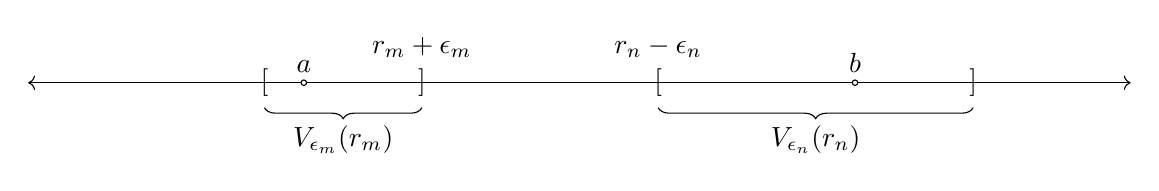
\begin{tikzpicture}
                \draw[<->] (-7, 0) -- (7, 0);
                \filldraw[draw=black, fill=white]
                    (-3.5, 0) circle (1pt) node [anchor=south] {\( a \)}
                    (3.5, 0) circle (1pt) node [anchor=south] {\( b \)};
                \path
                    (-4, 0) node {[}
                    (-2, 0) node {]}
                    (-2, 0) node [anchor=south, yshift=2mm] {\( r_m + \epsilon_m \)}
                    (1, 0) node {[}
                    (1, 0) node [anchor=south, yshift=2mm] {\( r_n - \epsilon_n \)}
                    (5, 0) node {]};
                \draw[decorate, decoration = {brace, raise = 9, amplitude = 4}] (-2, 0) -- (-4, 0) node [pos = 0.5, below = 12] {\( V_{\epsilon_m}(r_m) \)};
                \draw[decorate, decoration = {brace, raise = 9, amplitude = 4}] (5, 0) -- (1, 0) node [pos = 0.5, below = 12] {\( V_{\epsilon_n}(r_n) \)};
            \end{tikzpicture}
            \caption{\( V_{\epsilon_m}(r_m) \) and \( V_{\epsilon_n}(r_n) \)} \label{fig:2}
        \end{figure}
        
        Thus \( r_m + \epsilon_m \in (a, b) \subseteq (x - \delta, x) \subseteq O \). There then exists a \( k \in \N \) such that \( r_m + \epsilon_m \) belongs to \( V_{\epsilon_k}(r_k) \). If \( k = m \), this says that an open interval contains one of its endpoints, which is a contradiction, and if \( k \neq m \) then this violates (A3).

        Thus if an interval such as \( (x - \delta, x) \) is to be contained in \( O \), it must be entirely contained inside a single \( V_{\epsilon_n}(r_n) \). Then since \( (x - \delta, x) \) and \( (x, x + \delta) \) are disjoint, there exist \( m, n \in \N \) with \( m \neq n \) such that
        \[
            (x - \delta, x) \subseteq V_{\epsilon_m}(r_m) \quand (x, x + \delta) \subseteq V_{\epsilon_n}(r_n).
        \]
        This implies that
        \[
            [x - \delta, x] \subseteq \overline{V_{\epsilon_m}(r_m)} \quand [x, x + \delta] \subseteq \overline{V_{\epsilon_n}(r_n)},
        \]
        which in turn gives \( x \in \overline{V_{\epsilon_m}(r_m)} \cap \overline{V_{\epsilon_n}(r_n)} \), contradicting (A3). We may conclude that \( F \) is a perfect set.
    \end{enumerate}
\end{solution}

\noindent \hrulefill

\noindent \hypertarget{ua}{\textcolor{blue}{[UA]} Abbott, S. (2015) \textit{Understanding Analysis.} 2\ts{nd} edition.}

\end{document}